%%%%%%%%%%%%%%%%%%%%%%%%%%%%%%%%%%%%%%%%%
% Beamer Presentation
% LaTeX Template
% Version 1.0 (10/11/12)
%
% This template has been downloaded from:
% http://www.LaTeXTemplates.com
%
% License:
% CC BY-NC-SA 3.0 (http://creativecommons.org/licenses/by-nc-sa/3.0/)
%
%%%%%%%%%%%%%%%%%%%%%%%%%%%%%%%%%%%%%%%%%

%----------------------------------------------------------------------------------------
%	PACKAGES AND THEMES
%----------------------------------------------------------------------------------------

\documentclass{beamer}

\mode<presentation> {

% The Beamer class comes with a number of default slide themes
% which change the colors and layouts of slides. Below this is a list
% of all the themes, uncomment each in turn to see what they look like.

%\usetheme{default}
%\usetheme{AnnArbor}
%\usetheme{Antibes}
% \usetheme{Bergen}
%\usetheme{Berkeley}
%\usetheme{Berlin}
%\usetheme{Boadilla}
%\usetheme{CambridgeUS}
%\usetheme{Copenhagen}
%\usetheme{Darmstadt}
%\usetheme{Dresden}
% \usetheme{Frankfurt}
%\usetheme{Goettingen}
% \usetheme{Hannover}
%\usetheme{Ilmenau}
%\usetheme{JuanLesPins}
%\usetheme{Luebeck}
\usetheme{Madrid}
%\usetheme{Malmoe}
% \usetheme{Marburg}
%\usetheme{Montpellier}
%\usetheme{PaloAlto}
% \usetheme{Pittsburgh}
%\usetheme{Rochester}
% \usetheme{Singapore}
%\usetheme{Szeged}
%\usetheme{Warsaw}

% As well as themes, the Beamer class has a number of color themes
% for any slide theme. Uncomment each of these in turn to see how it
% changes the colors of your current slide theme.

%\usecolortheme{albatross}
%\usecolortheme{beaver}
%\usecolortheme{beetle}
%\usecolortheme{crane}
%\usecolortheme{dolphin}
%\usecolortheme{dove}
%\usecolortheme{fly}
%\usecolortheme{lily}
%\usecolortheme{orchid}
%\usecolortheme{rose}
%\usecolortheme{seagull}
%\usecolortheme{seahorse}
%\usecolortheme{whale}
%\usecolortheme{wolverine}

%\setbeamertemplate{footline} % To remove the footer line in all slides uncomment this line
%\setbeamertemplate{footline}[page number] % To replace the footer line in all slides with a simple slide count uncomment this line

%\setbeamertemplate{navigation symbols}{} % To remove the navigation symbols from the bottom of all slides uncomment this line
}

\usepackage{graphicx} % Allows including images
\usepackage{booktabs} % Allows the use of \toprule, \midrule and \bottomrule in tables

%----------------------------------------------------------------------------------------
%	TITLE PAGE
%----------------------------------------------------------------------------------------

\title[EMSE - Stage]{Implementation of a Robot Behaviour Learning Simulator} % The short title appears at the bottom of every slide, the full title is only on the title page

\author{Kushagra Singh Bisen} % Your name
\institute[EMSE] % Your institution as it will appear on the bottom of every slide, may be shorthand to save space
{
Ecole des Mines de Saint Etienne \\ % Your institution for the title page
\medskip
\textit{Master 1 Defence} % Your email address
}
\logo{

\includegraphics[width=1cm]{images/EMSE_logo.png}
% \hspace{2cm}
% 
\includegraphics[width=3cm]{images/UJM_logo.png}
}
\date{\today} % Date, can be changed to a custom date

\begin{document}

\begin{frame}
\titlepage % Print the title page as the first slide
\end{frame}

\begin{frame}
\frametitle{Overview} % Table of contents slide, comment this block out to remove it
\tableofcontents % Throughout your presentation, if you choose to use \section{} and \subsection{} commands, these will automatically be printed on this slide as an overview of your presentation
\end{frame}

%----------------------------------------------------------------------------------------
%	PRESENTATION SLIDES
%----------------------------------------------------------------------------------------

\section{Context and Motivation}
\begin{frame}
    \Huge{\centerline{Context and Motivation}}
\end{frame}

\begin{frame}
    \frametitle{Lab Overview}

    \begin{itemize}
        \item Department of Computing and Intelligent Systems is situated in Institut Henri Fayol, EMSE.
        \item The department aims to develop algorithms and architectures for the interconnection of physical, digital and social worlds.
        \item The interconnection takes in account of all the dimensions neccesary for the deployment of applications in Industry 4.0 and Smart Cities.
        \item The department's research interests lie in knowledge representation, reasoning, multi agent system, data mining and security.
    \end{itemize}
\end{frame}

\begin{frame}
    \frametitle{Motivation}
    \begin{itemize}
        \item The work is based in an Industry 4.0 scenario.
        \item There are various entities in the environment, both mobile and static.
        \item We wish to study and record the behaviour of the robot while it moves.
        \item The behaviour of the robot is used to detect and prevent collisions.
        \item The work will be included in the Set of Intelligent Robots project at Institut Henri Fayol.
    \end{itemize}
\end{frame}

\begin{frame}
    \frametitle{Robot}
    \begin{itemize}
        \item  A system with decision making capabilities.
        \item  A Cyber-Physical System (CPS) combining sensing, actuation and computation.
        \item  Perform Dirty, Dull or Dangerous tasks.
        \item  Various applications, as \textit{mobility on demand}, \textit{drone servillance}, \textit{long distance logistics} and \textit{automated highways}
    \end{itemize}
\end{frame}

\begin{frame}
    \frametitle{Essential Qualities of Robot}
    Autonomy is essential for a system to be called a robot.
    Autonomy is achieved through,
    \begin{itemize}
        \item Perception \label{Perception} : employing \textit{proprioceptive sensors} and \textit{exteroceptive sensors}
        \item Action \label{Action} : calculation of velocities to move in a direction.
        \item Decision Making : Utilizes previous modules to result in \textit{navigation}
    \end{itemize}
\end{frame}

\begin{frame}
    \frametitle{Digital Twins}
    \begin{itemize}
        \item Model an Industry 4.0 process/machine.
        \item Enabling testing, training and error detection before real-life implementation.
        \item Defined as machines which are simulating, mirroring, and "twinning" a physical entity.
        \item It can be linked to a \textit{physical twin} \cite{p2}
        \item It is not a \textbf{simulation} but an exact replica of it's \textbf{physical twin}.
        \item enabling communication-collaboration-interaction with PT (physical twin)
        \item a part of Cyber-Physical Systems.
    \end{itemize}
\end{frame}

\begin{frame}
    \frametitle{Behavioural Learning}
    \begin{itemize}
        \item Learning the behaviour of the robot in the space.
        \item The behaviour of the robot can be learnt by it's position as well as it's position relative to the obstacles.
        \item The behaviour of the robot is used for reinforcement learning.
    \end{itemize}
\end{frame}

\begin{frame}
    \frametitle{Objectives}
    \textbf{Implementation Questions}
    \begin{itemize}
        \item How can we make the robot move from a position to the other?
        \item How can we represent the configuration space in simulator?
        \item Which data can \textit{we use/not use} for behaviour learning?
        \item Which method we can use for behaviour learning?
    \end{itemize}
\end{frame}

\section{Implementation}

\begin{frame}
    \Huge{\centerline{Implementation}}
\end{frame}

\begin{frame}
    \frametitle{Technologies}
    \begin{itemize}
        \item \textbf{Turtlebot} : Personal robot kit with LIDAR sensor running on open-source software.
        \item \textbf{Gazebo Simulator} \cite{p3} : Used to visualise the Turtlebot and the environment generated by 3D models.
        \item \textbf{Robot Operating Systems} : flexible framework which provides abstraction, libraries, drivers, package management.
    \end{itemize}
\end{frame}

\begin{frame}
    \frametitle{Simultaneous Localization and Mapping (SLAM)}
    \begin{itemize}
        \item Technique for self-exploration of the environment.
        \item Fundamental requirement for an autonomous system.
        \item Combines two different technologies, i.e Localization and Mapping.
        \item It is done concurrently as the robot moves.
    \end{itemize}
\end{frame}

\begin{frame}
    \frametitle{Features of SLAM}
    \begin{itemize}
        \item \textbf{Localization} : Using odometry information of the robot to estimate the position in environment.
        \item \textbf{Mapping} : Using the LIDAR sensor to register information (obstacles and position) about the environment producing a map file.
    \end{itemize}
\end{frame}

\begin{frame}
    \frametitle{SLAM Workflow}
    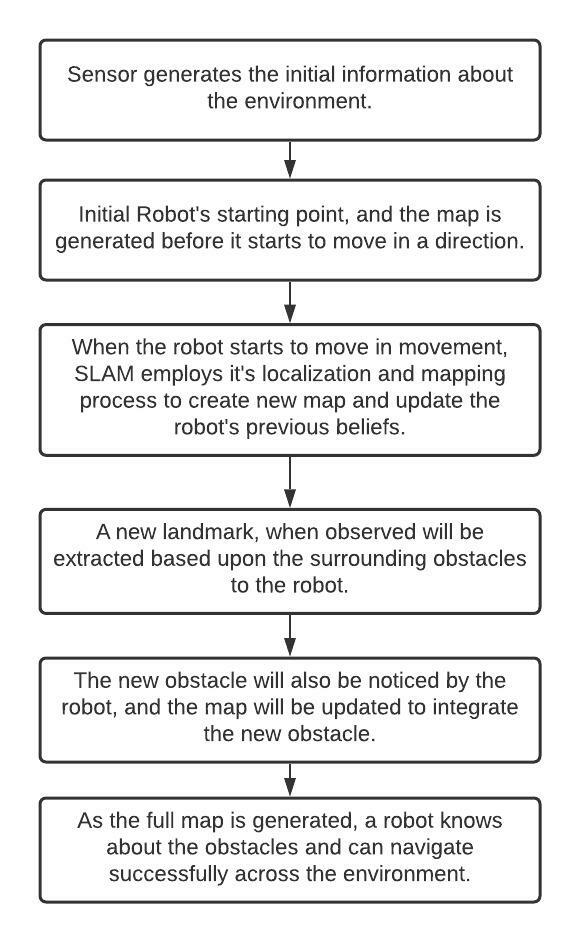
\includegraphics[width=6cm, height=8.5cm]{images/SLAM_flowchart.jpeg}
\end{frame}

\begin{frame}
    \frametitle{Step-By-Step SLAM}
    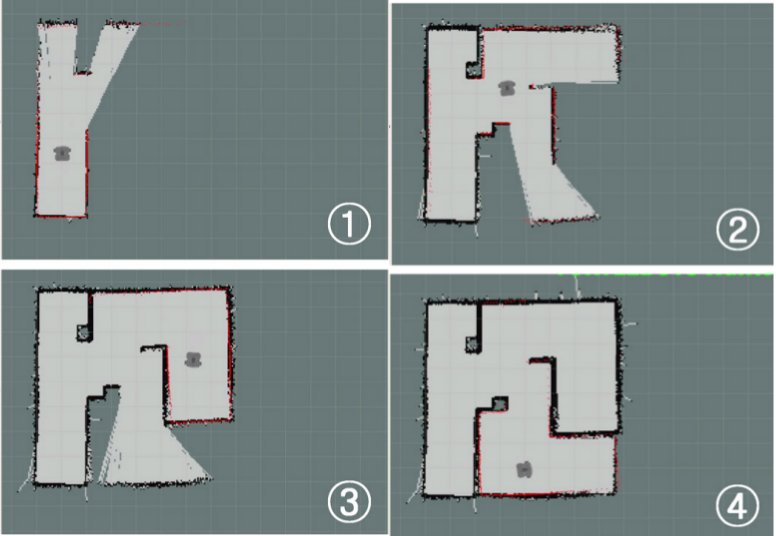
\includegraphics[width=0.8\textwidth]{images/SLAM.png}
\end{frame}

\begin{frame}
    \frametitle{Path Planning Algorithms}
    Path Planning Algorithms provide methods to execute planning to the goal state. They are of two types : 
    \begin{itemize}
        \item \textit{Global Planner Algorithms} : Offline algoritms to calculate further states of the robot. Implemented algorithms are, \textit{Dijkstra}, \textit{A*} and Greedy Best First Search Algorithm.
        \item \textit{Local Planner Algorithms} : Online dynamic algoritms to calculate the path while the robot is moving. Implemented algorithm is, \textit{Dynamic Window Approach Planner}. 
    \end{itemize}
\end{frame}

\begin{frame}
    \frametitle{Exploration Stage 1}
    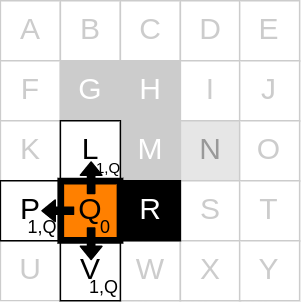
\includegraphics[width=0.5\textwidth]{images/grid_map_expansion_02.png}
\end{frame}

\begin{frame}
    \frametitle{Exploration Stage 2}
    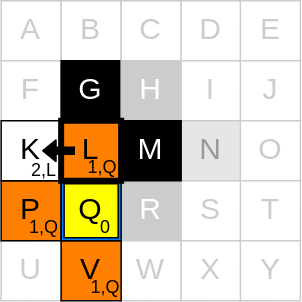
\includegraphics[width=0.5\textwidth]{images/grid_map_expansion_03.png}
\end{frame}

\begin{frame}
    \frametitle{Dynamic Window Approach Algorithm}
    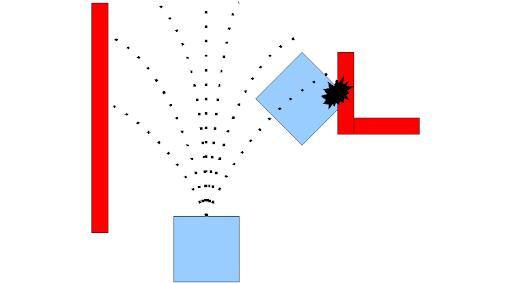
\includegraphics[width=\textwidth]{images/dwa_planner.png}
\end{frame}

\begin{frame}
    \frametitle{Navigation Implementation}
    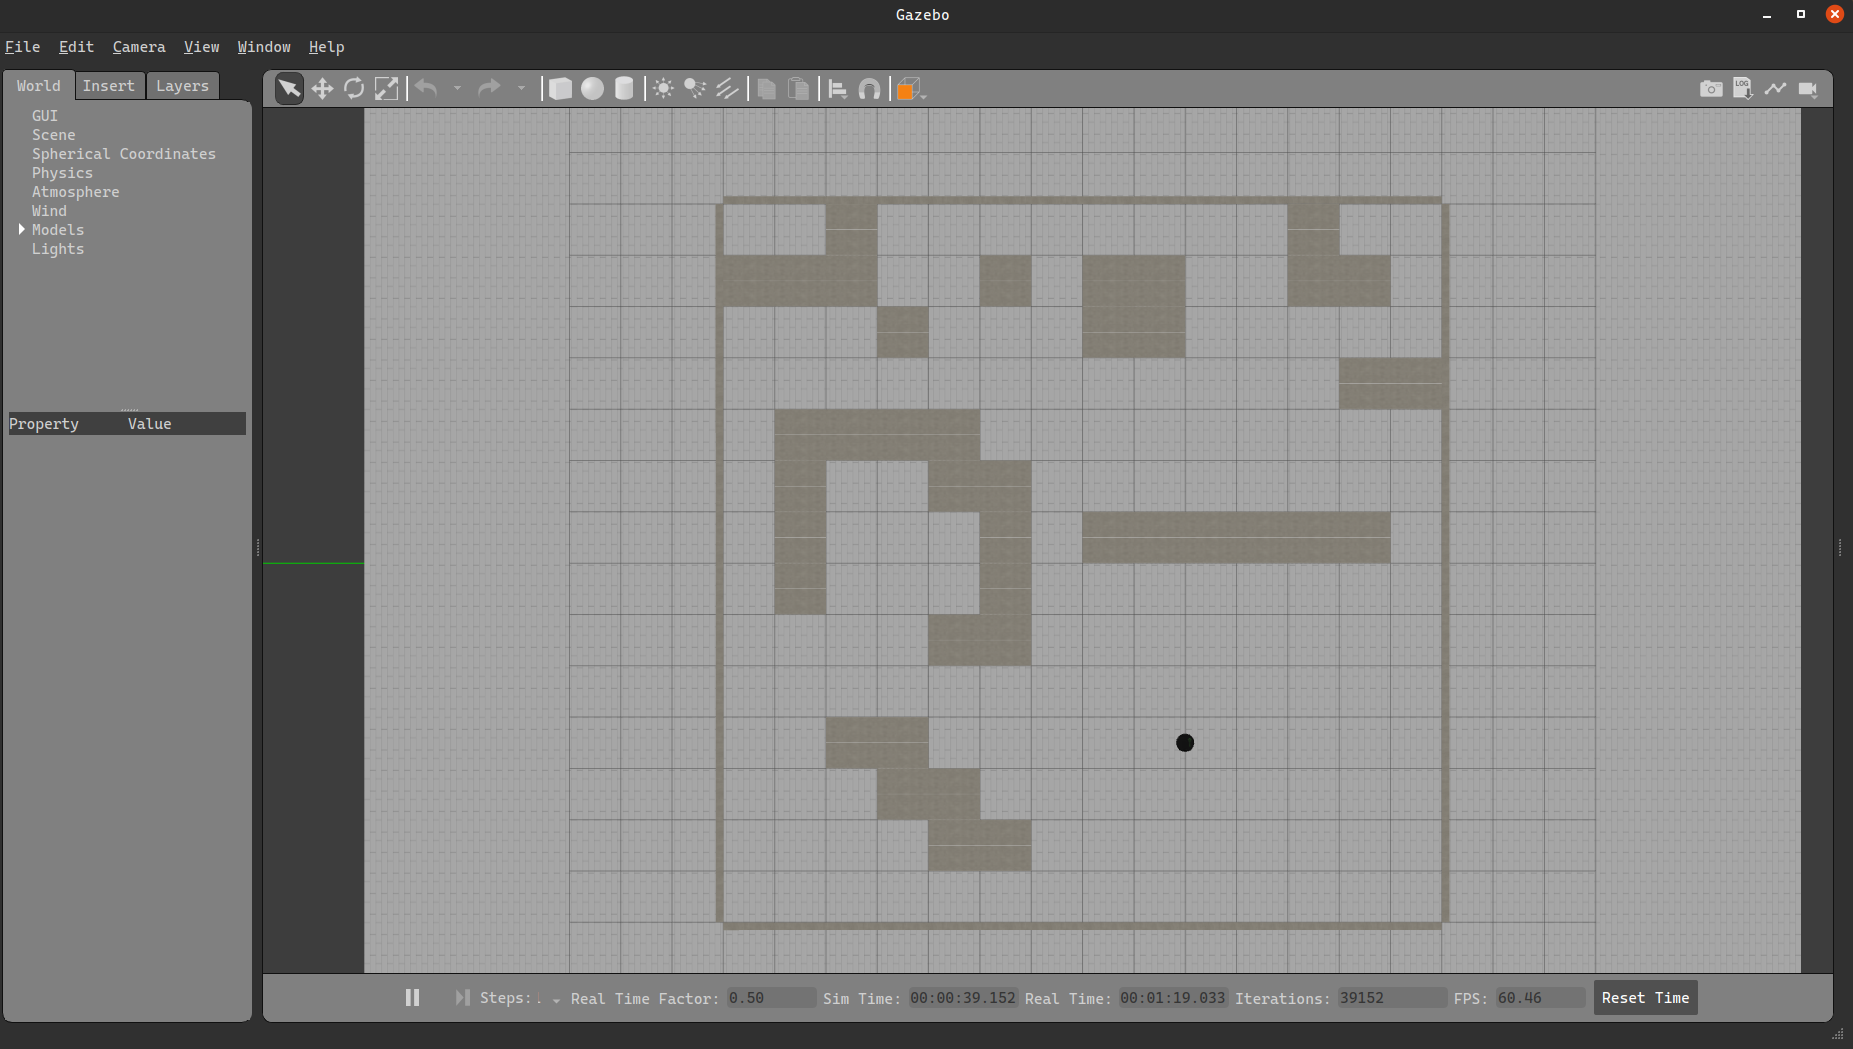
\includegraphics[width=\textwidth]{images/base_god_eye_world.png}
\end{frame}

\begin{frame}
    \frametitle{Navigation Implementation (Contd.)}
    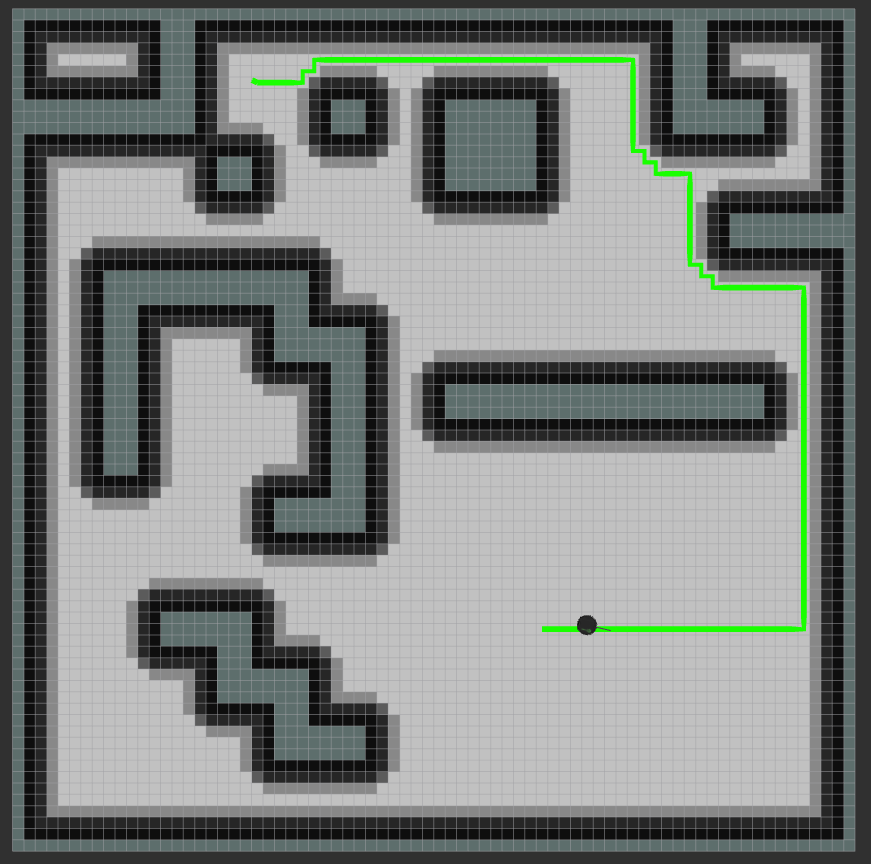
\includegraphics[width=0.7\textwidth]{images/RVIZ-Grid.png}
\end{frame}

\begin{frame}
    \frametitle{Method for Behaviour Learning}
    The hypothesis is to use the digital twin made to store the information related to
    the state and neighborhood of the robot by \textit{God's Eye} 

    \begin{figure}
        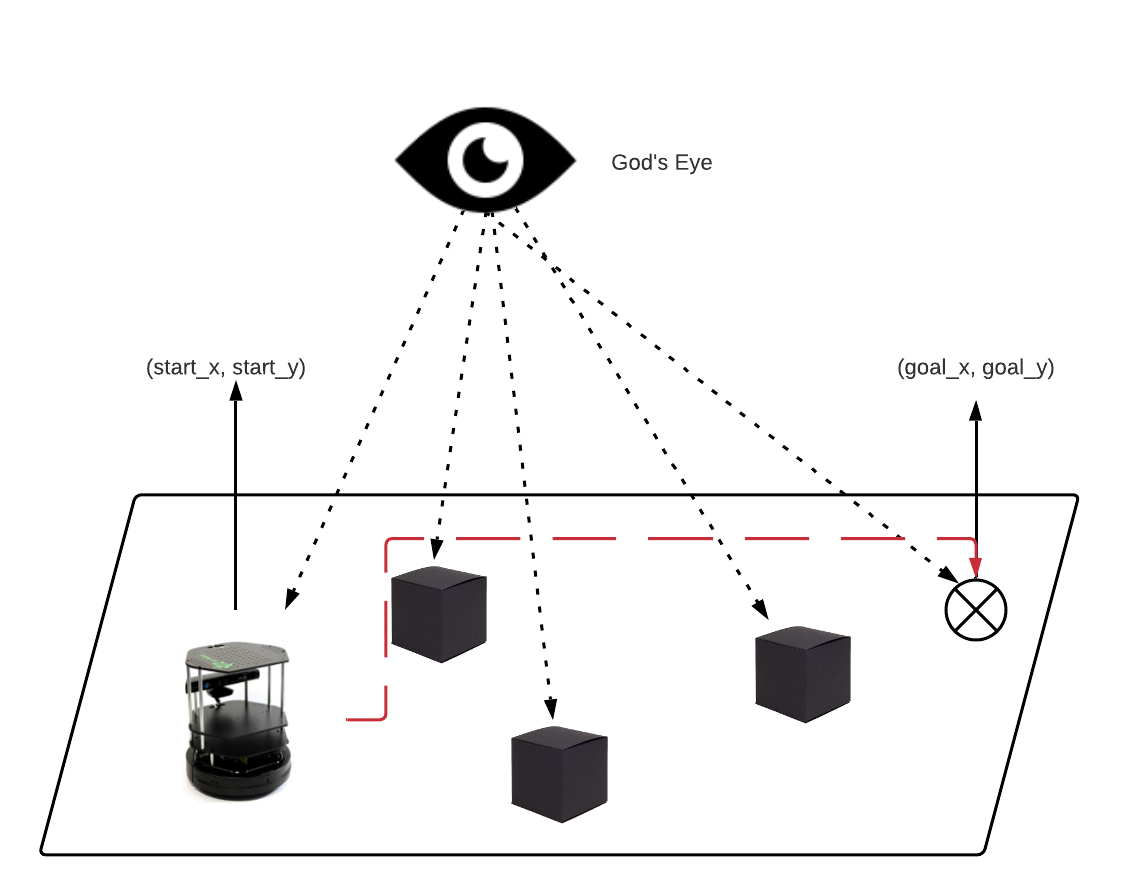
\includegraphics[width=0.7\textwidth]{images/God-eye.png}
    \end{figure}
\end{frame}

\begin{frame}
    \frametitle{Method (Contd.)}
    \begin{itemize}
        \item Each obstacle is represented by a pair of x and y coordinates.
        \item The x and y coordinates of robot can be infered by odometry.
        \item A distance or a \textit{fake perception range} is specified to construct the grid.
        \item Grid's positions are calculated by adding the perception range to the coordinate.
        \item If they are equal, an obstacle is recorded.
        \item The obstacle behaviour grid is record and stored.
    \end{itemize}
\end{frame}

\begin{frame}
    \frametitle{Method (Contd.)}
    \begin{itemize}
        \item We had to divide the obstacle coordinate into more coordinate points for better accuracy in the grid space.
        \item One obstacle is represented by not one, but 72 coordinate points.
        \item The individual grid size is 0.1, and it can be changed as per the requirement.
        \item The grid space calculated is of sizes 3 by 3, 5 by 5, 7 by 7 and further with the robot in middle.
        \item Bigger Grid Size shows better information of the robot's space.
    \end{itemize}

    \begin{figure}
        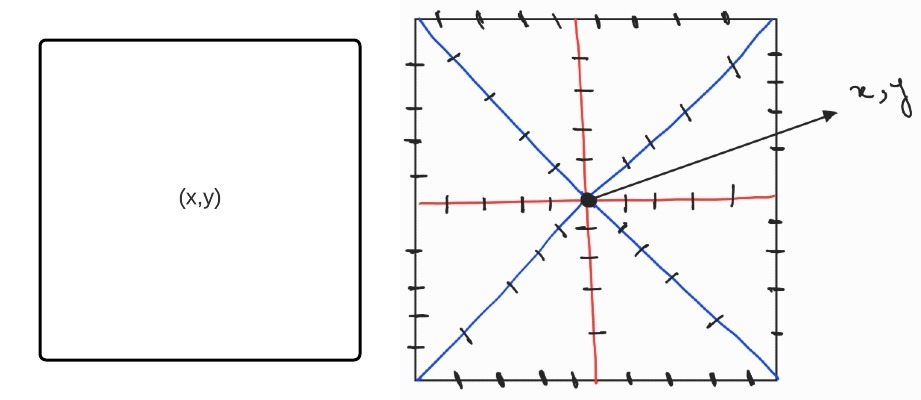
\includegraphics[width=0.8\textwidth]{images/obstacle-grid.jpg}
    \end{figure}
\end{frame}

\begin{frame}
    \frametitle{Generated Log}
    The generated log file in semi structed data format contains,
    \begin{itemize}
        \item Timestamp in seconds.
        \item x, y coordinates of the robot.
        \item obstacle grid.
        \item x,y coordinates of the goal.
        \item relative coordinates to the goal.
        \item manhattan distance to the goal.
        \item euclidian distance to the goal.
        \item angular rotation of the robot.
    \end{itemize}
\end{frame}

\section{Conclusion}

\begin{frame}
    \Huge{\centerline{Conclusion}}
\end{frame}

\begin{frame}
    \frametitle{Conclusion}
    To summarize, we developed
    \begin{itemize} 
        \item a digital twin for autonomous behaviour of robot by avoiding obstacles to a goal.
        \item a method for generating a static grid for neighborhood space.
    \end{itemize}
    On-going and future work,
    \begin{itemize}
        \item Implementing the method in different scenarios of the environment.
        \item Implementing multiple robots to form a multiple robot system and recording behaviour for each.
        \item The recorded behaviour can be used for machine learning, training, and testing to develop stratey with digital twins.
        \item Robot's arm i.e a Manipulator's Behaviour can be studied in future.
    \end{itemize}
\end{frame}




%------------------------------------------------
\begin{frame}
\Huge{\centerline{Thank you for your time.}}
\end{frame}

\begin{frame}
    \frametitle{References}
    \footnotesize{
    \begin{thebibliography}{99} % Beamer does not support BibTeX so references must be inserted manually as below
   \bibitem[B. R. Barricelli, E. Casiraghi and D. Fogli, 2019]{p2} Barricelli et al. (2019)
   \newblock A Survey on Digital Twin: Definitions, Characteristics, Applications, and Design Implications
   \newblock \emph{IEEE Access}, vol. 7, pp. 167653-167671, 2019, doi: 10.1109/ACCESS.2019.2953499

    \bibitem[Koenig, N. and Howard, A.]{p3} Koenig et al. (2004)
    \newblock Design and use paradigms for Gazebo, an open-source multi-robot simulator
    \newblock \emph{2004 IEEE/RSJ International Conference on Intelligent Robots and Systems (IROS) (IEEE Cat. No.04CH37566)}

    \end{thebibliography}
    }
\end{frame}

%----------------------------------------------------------------------------------------

\end{document} 